\documentclass[12pt, a4paper, oneside]{ctexart}
\usepackage{amsmath, amsthm, amssymb, graphicx}
\usepackage[bookmarks=true, colorlinks, citecolor=blue, linkcolor=black]{hyperref}
\usepackage[margin = 25mm]{geometry}
\usepackage{setspace}
% 导言区
\title{双delta势垒}
\date{\today}
\author{欸嘿}
\begin{document}
\begin{spacing}{2.0}
\maketitle
\section{双delta势}
现在假设有一势$V=\alpha[\delta(x+a)+\delta(x-a)]$
\begin{figure}[htbp]
    \centering
    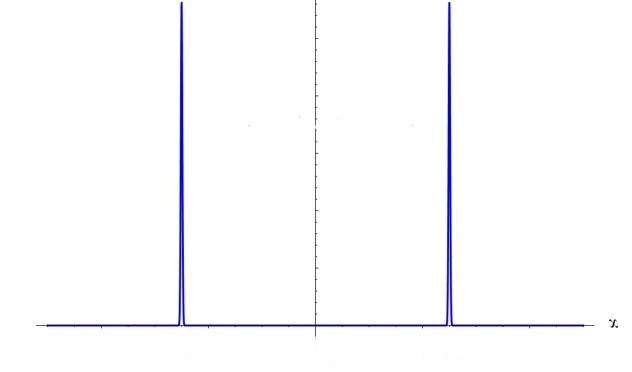
\includegraphics[width=8cm]{delta.jpg}
    \caption{$V=\alpha[\delta(x+a)+\delta(x-a)]$}
\end{figure}
\subsection{求解}
\begin{center}
对于薛定谔方程:\\
$i\hbar\frac{\partial \Psi}{\partial t} = -\frac{\hbar^2}{2 m} \frac{\partial^2 \Psi}{\partial x^2}+V(x) \Psi(x,t)$\\
分离变量 $\Psi(x,t)=\psi(x)\phi(t)$\\
$i\hbar\psi\frac{d\phi}{dt}=-\frac{\hbar^2}{2m} \phi\frac{d^2 \psi}{dx^2}+V\psi\phi$\\
$\Rightarrow i\hbar\frac{\dot\phi}{\phi}=-\frac{\hbar^2}{2m}\frac{\ddot\psi}{\psi}+V=E $\\
$\left\{\begin{matrix}    i\hbar\frac{\dot\phi}{\phi}=E \\     -\frac{\hbar^2}{2m}\frac{\ddot\psi}{\psi}+V=E  \end{matrix}\right. $\\
\end{center}
\begin{center}
将势能V带入,得
$\left\{\begin{matrix}    i\hbar\frac{\dot\phi}{\phi}=E \\     -\frac{\hbar^2}{2m}\frac{\ddot\psi}{\psi}+\alpha[\delta(x+a)+\delta(x-a)]=E  \end{matrix}\right. $\\
E为满足边界条件的特征值,\\
$ \frac{\partial^2\psi}{\partial x^2}-\frac{2m}{\hbar^2} \left\{\alpha[\delta(x+a)+\delta(x-a)]-E\right\}\psi=0$   (1)\\
如果$x\neq \pm a$,
$\Rightarrow \frac{\partial^2\psi}{\partial x^2}+\frac{2mE}{\hbar^2}\psi=0 $
会有以下解\\
$\psi(x)= \left\{\begin{matrix}    Ae^{kx},x<-a \\    Ce^{kx}+De^{-kx},-a<x<a\\Fe^{-kx},x>a\\  \end{matrix}\right. ,k=\frac{\sqrt{-2mE}}{\hbar}$\\
并且此时有边界条件:\\
$ \lim\limits_{x \to -a^-}\psi(x)=\lim\limits_{x \to -a^+}\psi(x)$\\
$ \lim\limits_{x \to +a^-}\psi(x)=\lim\limits_{x\to+a^+}\psi(x)$\\
这样可得:
$\left\{\begin{matrix} Ae^{-ka}=Ce^{-ka}+De^{ka}\\ Fe^{-ka}=Ce^{ka}+De^{-ka}\end{matrix}\right. $\\
而其他的条件可对(1)式积分,范围从$-a-\epsilon$到$-a+\epsilon$\\
$\displaystyle\int^{-a+\epsilon}_{-a-\epsilon}\left\{\frac{\partial^2\psi}{\partial x^2}-\frac{2m}{\hbar^2} \left\{\alpha[\delta(x+a)+\delta(x-a)]+E\right\}\psi\right\} dx=0 $\\
$\displaystyle\int^{-a+\epsilon}_{-a-\epsilon}\frac{\partial^2\psi}{\partial x^2}dx-\frac{2m}{\hbar^2}\left\{\alpha\displaystyle\int^{-a+\epsilon}_{-a-\epsilon}[\delta(x+a)+\delta(x-a)]\psi(x) dx+E \displaystyle\int^{-a+\epsilon}_{-a-\epsilon}\psi(x) dx\right\}=0$\\
$\frac{\mathrm{d}\psi}{\mathrm{d}x}\bigg|^{a+\epsilon}_{a-\epsilon}-\frac{2m}{\hbar^2}\bigg[\alpha\psi(a)+E\psi(a)\displaystyle\int^{a+\epsilon}_{a-\epsilon}\mathrm{d}x\bigg]=0$\\
$\frac{\mathrm{d}\psi}{\mathrm{d}x}\bigg|^{a+\epsilon}_{a-\epsilon}-\frac{2m}{\hbar^2}[\alpha\psi(a)+E\psi(a)(2\epsilon)]=0$ , 令$\epsilon \to 0$\\
$\frac{\mathrm{d}\psi}{\mathrm{dx}}\bigg|^{-a^+}_{-a^-}-\frac{2m\alpha}{\hbar^2}\psi(-a)=0$\\
$\frac{2m\alpha}{\hbar^2}\psi(-a)=\lim\limits_{x \to -a^-}\frac{\mathrm{d}\psi}{\mathrm{d}x}-\lim\limits_{x \to -a^+}\frac{\mathrm{d}\psi}{\mathrm{d}x}$\\
$\frac{2m\alpha}{\hbar^2}Fe^{-ka}=\biggl[kCe^{ka}-kDe^{-ka}+kFe^{-ka}\biggl]$\\
\end{center}
这样就有四个条件可以求解了,
$\left\{\begin{matrix} Ae^{-ka}=Ce^{-ka}+De^{ka}\\ Fe^{-ka}=Ce^{ka}+De^{-ka}\\\frac{2m\alpha}{\hbar^2}Fe^{-ka}=\biggl[kCe^{ka}-kDe^{-ka}+kFe^{-ka}\biggl]\\\frac{2m\alpha}{\hbar^2}Ae^{-ka}=\biggl[kAe^{-ka}-kCe^{-ka}+kDe^{ka}\biggl]\end{matrix}\right. $\\
最终可以得到\\
$D=(\frac{\hbar^2 k}{m\alpha}-1)^2De^{4ka}$\\
$1=(\frac{\hbar^2 k}{m\alpha}-1)e^{2ka}$\\
$\left\{\begin{matrix} \frac{k\hbar^2}{m\alpha}-1=e^{-2ka}, even \\ 1-\frac{k\hbar^2}{m\alpha}=e^{-2ka},  odd\end{matrix}\right.  $\\


\end{spacing}
\end{document}
